\documentclass{beamer}

\usepackage{mathtext}
\usepackage{ucs}
\usepackage[utf8x]{inputenc}
\usepackage[T2A]{fontenc}
\usepackage[english,ukrainian]{babel}
\usepackage{amsfonts,amsmath,stmaryrd}
\usepackage{textcomp}
\usepackage{float}
\usepackage{wrapfig} 

\usepackage{ucs}
\usepackage[utf8x]{inputenc}
\usepackage[T2A]{fontenc}
\usepackage[english,ukrainian]{babel}

\usetheme{JuanLesPins}
\usefonttheme[]{serif}

\title{Курсова робота}
\subtitle{на тему: \\
\large{\textbf{Індуктивні методи самоорганізації агента в задачах навігації}}}

\author{Накрийко Андрій}
\institute{Львівський національний університет ім. І.Франка}

\date{Львів - 2009}

\begin{document}
\frame{\titlepage}

\frame{
\frametitle{\textbf{Постановка задачі навігації агента}}
\Large
\begin{itemize}
\item базується на обмеженій інформації про середовище
\item обмежений набір допустимих дій
\item добирання до вказаної цілі
\item уникнення зіткнення з перешкодами
\item якомога менша кількість ходів 
\end{itemize}
}

\frame{
\frametitle{\textbf{Дедуктивні та індуктивні методи навчання}}
\Large
Попередній дедуктивний підхід:
\begin{itemize}
\item система експертних правил
\item нейромережа як узагальнюючий елемент
\item складність створення репрезентативних правил
\end{itemize}

Індуктивний самоорганізаційний підхід:
\begin{itemize}
\item самостійне вироблення внутрішніх правил
\item ефективне використання набутого досвіду
\item толерантність до зміни структури сприйняття середовища
\end{itemize}
}

\frame{
\frametitle{\textbf{Парадигма навчання з підсиленням}}
\begin{figure}
\centering
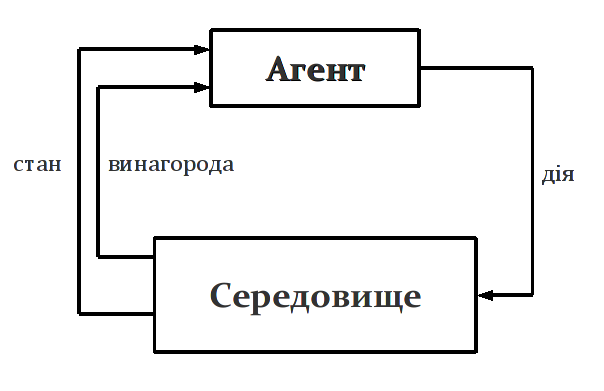
\includegraphics[width=0.8\textwidth]{agent_env_diagram.png}
\end{figure}
}

\frame{
\frametitle{\textbf{Алгоритм Sarsa}}
\begin{center}
	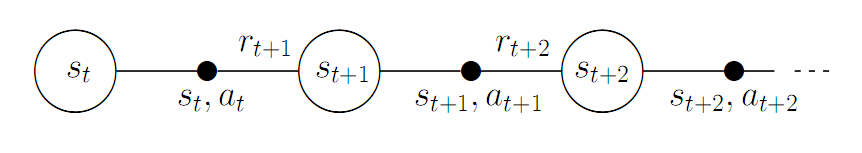
\includegraphics[width=0.9\textwidth]{sarsa_sequence.PNG}
	\begin{itemize}
		\item $Q(s_t,a_t) \leftarrow Q(s_t,a_t) + \alpha\left[r_{t+1} + \gamma Q(s_{t+1},a_{t+1}) - Q(s_t,a_t)\right]$
		\item \Large{Стратегія вибору дії "--- \textit{$\varepsilon$-жадібна}}
		\item \Large{Нейромережа як універсальний апроксиматор функцій}
	\end{itemize}
\end{center}
}

\frame{
\frametitle{\textbf{Сприйняття агентом середовища}}
\begin{center}
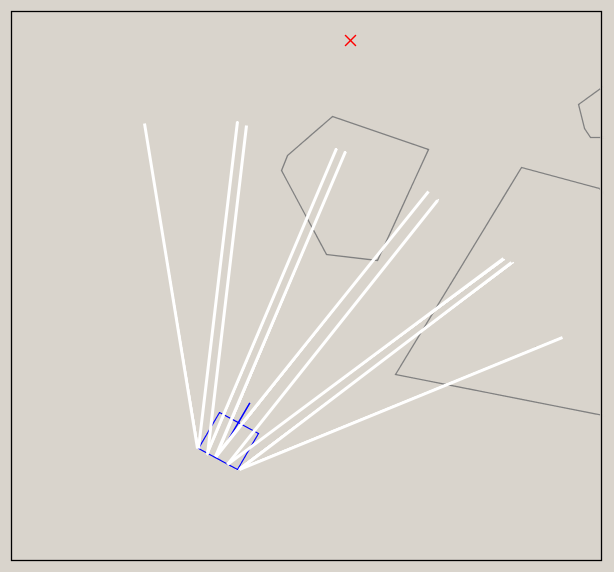
\includegraphics[width=0.7\textwidth]{perception.png}
%\begin{itemize}
%	\item 5 секторів сприйняття перешкод
%	\item відстань до цілі
%	\item кут на напрямок до цілі
%	\item обмеженість дальності огляду
%\end{itemize}
\end{center}
}

\frame{
\frametitle{Процес навчання}
\Large
\begin{itemize}
\item Епізодичне навчання
\item Випадкова конфігурація кімнати
\item Покарання та винагороди за кожен хід
\item Зміна ймовірності вибору випадкової дії
\end{itemize}
}

\frame{
\frametitle{\textbf{Результати}}
\Large
\begin{itemize}
\item збіжність до оптимальної стратегії за 1.2 млн. кроків
\item успішне добирання до цілі у 87\%-92\% епізодів
\item незалежність від конкретного розташування перешкод та цілі
\item великі часові затрати на навчання
\item гнучкість підходу
\end{itemize}
}

\section{Приклад процесу навчання}
\frame{
\frametitle{\textbf{Приклад процесу навчання} \\ (початок навчання)}
\begin{figure}
\centering
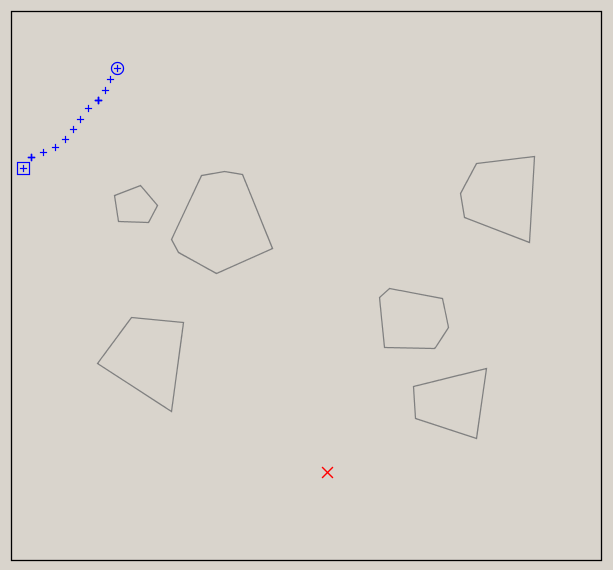
\includegraphics[width=0.65\textwidth]{learn1.png}
\end{figure}
}
\frame{
\frametitle{\textbf{Приклад процесу навчання} \\ (після 100 тис. кроків навчання)}
\begin{figure}
\centering
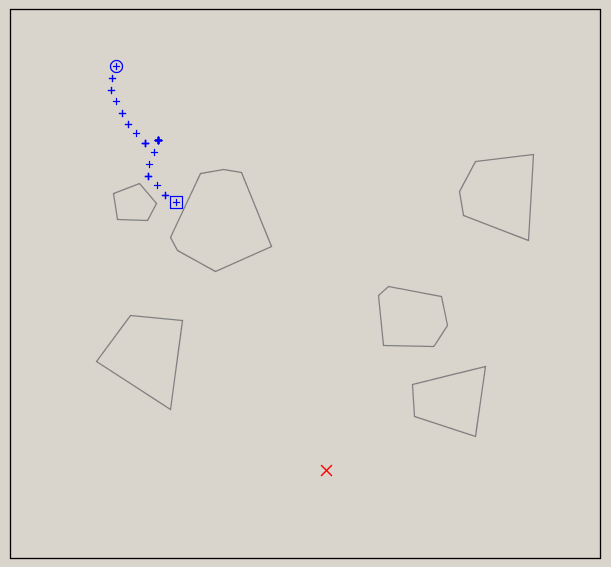
\includegraphics[width=0.65\textwidth]{learn2.png}
\end{figure}
}
\frame{
\frametitle{\textbf{Приклад процесу навчання} \\ (після 500 тис. кроків навчання)}
\begin{figure}
\centering
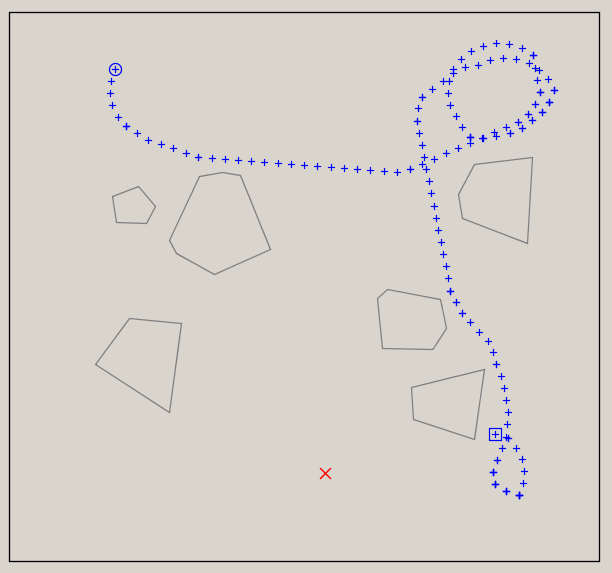
\includegraphics[width=0.65\textwidth]{learn3.png}
\end{figure}
}
\frame{
\frametitle{\textbf{Приклад процесу навчання} \\ (після 1.2 млн. кроків навчання)}
\begin{figure}
\centering
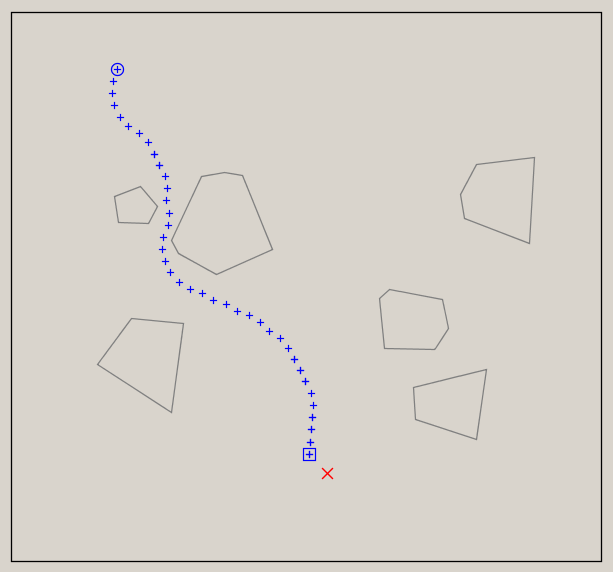
\includegraphics[width=0.65\textwidth]{learn4.png}
\end{figure}
}

\section{На завершення}
\frame{
\frametitle{Перспективи}
\Large
\begin{itemize}
\item зміна завдання агента на більш складне
\item введення в агента елементів пам'яті (динамічна побудова карти)
\item перехід до ієрархічного навчання
\end{itemize}
}
\frame{
\begin{center}\Huge{Запитання та зауваження?}\end{center}
}
\frame{
\begin{center}\Huge{\textbf{Дякую за увагу!}}\end{center}
}
\end{document} 